\documentclass[output=paper,colorlinks,citecolor=brown]{langscibook} 

\newcommand*{\fullref}[1]{\hyperref[{#1}]{\autoref*{#1}: \nameref*{#1}}} % One single link

%dependencias para desenhar árvores sintáticas
\usepackage{tikz}
\usepackage{tikz-dependency}
%\usepackage{python}
%\usepackage{minted} %\begin{minted}{python}
\usepackage{longtable}

%nome da section no header de cada página
%\usepackage{fancyhdr}
%\pagestyle{fancy}
%\fancyhf{}
%\fancyhead[L]{\rightmark}
%\fancyhead[R]{\thepage}
%\renewcommand{\headrulewidth}{0pt}
\usepackage{dirtytalk}

\bibliography{localbibliography.bib}

\author{Elvis de Souza\affiliation{PUC-Rio, Brasil}\and Tatiana Cavalcanti\and Aline Silveira\and Wograine Evelyn\and Cláudia Freitas}
\title{Documentação UD em português\\
(e para língua portuguesa)}
\abstract{O projeto Universal Dependencies \citep{mcdonald2013universal} apresenta um tagset \& uma gramática. Isso significa dizer que, para além de um conjunto de etiquetas que correspondem às classes da Gramática Tradicional (objeto, sujeito etc.), o UD também faz diversas escolhas que diferem da GT. Nesse documento, apresentamos a documentação detalhadas e as escolhas linguísticas relativas ao processo de revisão do material UD em Português. Considerando que UD funciona como uma espécie de segunda língua gramatical, partimos, sempre que possível, das categorias e análises de GT, e não de UD.}

% add all extra packages you need to load to this file  
\usepackage{tabularx} 

%%%%%%%%%%%%%%%%%%%%%%%%%%%%%%%%%%%%%%%%%%%%%%%%%%%%
%%%                                              %%%
%%%           Examples                           %%%
%%%                                              %%%
%%%%%%%%%%%%%%%%%%%%%%%%%%%%%%%%%%%%%%%%%%%%%%%%%%%% 
%% to add additional information to the right of examples, uncomment the following line
% \usepackage{jambox}
%% if you want the source line of examples to be in italics, uncomment the following line
% \renewcommand{\exfont}{\itshape}
\usepackage{langsci-optional}
\usepackage{langsci-gb4e}  
\makeatletter
\let\thetitle\@title
\let\theauthor\@author 
\makeatother

\newcommand{\togglepaper}[1][0]{ 
%   \bibliography{../localbibliography}
  \papernote{\scriptsize\normalfont
    \theauthor.
    \thetitle. 
    To appear in: 
    Change Volume Editor \& in localcommands.tex 
    Change volume title in localcommands.tex
    Berlin: Language Science Press. [preliminary page numbering]
  }
  \pagenumbering{roman}
  \setcounter{chapter}{#1}
  \addtocounter{chapter}{-1}
}

\begin{document}

\maketitle

\addtocontents{toc}{\protect\hypertarget{toc}{}}

\tableofcontents

\chapter{Formato UD}\label{sec:formatoud}

\hyperlink{toc}{Ir para tabela de conteúdos\\}

Os treebanks adaptados para a gramática UD são disponibilizados no formato CoNLL, em que há um token por linha. Cada anotação de cada token, por sua vez, é disposta em uma coluna, sendo 10 colunas ao todo. Cada token tem a configuração conforme a \fullref{tab:colunasUD}, com uma tabulação (\textit{Tab}) separando as colunas. Colunas sem nenhum valor devem, necessariamente, ser preenchidas com \textit{underline}.

\begin{table}
    \centering
    \begin{tabular}{c c c c c c c c c c}
        id & word & lemma & upos & xpos & feats & dephead & deprel & deps & misc\\
    \end{tabular}
    \caption{Colunas do formato UD 2.0}
    \label{tab:colunasUD}
\end{table}

\section{Colunas/anotações}\label{sec:colunas}



\begin{enumerate}
    \item “id” corresponde ao número do token, em ordem crescente;
    \item “word”, à palavra tal como aparece na frase (exceto no caso de contração, como “da”, em que a palavra será desmembrada nos tokens “de” e “a”);
    \item “lemma” se refere à palavra tal como aparece no dicionário: em no singular e em masculino ou infinitivo;
    \item “upos” (classe gramatical "universal") se refere à classe gramatical;
    \item No corpus Bosque-UD, a coluna “xpos” (classe gramatical específica) é preenchida com a saída do sistema PALAVRAS para a mesma frase;
    \item “feats” (atributos morfológicos) é preenchida com as características morfológicas do token;
    \item “dephead” (dependência sintática), com o id do token de quem é filho;
    \item “deprel” (relação de dependência), com a relação sintática que o conecta ao seu pai;
    \item “deps” (dependência específica) não é utilizado no Bosque-UD;
    \item “misc” (miscelânea) se refere a quaisquer informações extras que desejemos adicionar ao token.
\end{enumerate}{}

\section{Manipulação em Python}\label{sec:python}



Para manipular arquivos no formato UD em Python, com as classes Corpus, Sentence e Token (e suas respectivas anotações), desenvolvemos e utilizamos o \href{https://github.com/alvelvis/ACDC-UD/blob/master/estrutura_ud.py}{estrutura\_ud.py}.

\chapter{Classes gramaticais (upos)}\label{sec:upos}

\hyperlink{toc}{Ir para tabela de conteúdos\\}



As classes gramaticais em UD podem ser consultadas na \fullref{tab:upos}.

\begin{table}[]
    \centering
    \begin{tabular}{| c | c |}
    \hline
    \textbf{upos} & \textbf{Observações} \\
    \hline
    ADJ & adjetivos e numerais ordinais \\
    \hline
    ADP & preposições \\
    \hline
    PUNCT & pontuação \\
    \hline
    ADV & advérbio \\
    \hline
    AUX & auxiliar - \say{ser}, \say{estar} (\fullref{sec:verbosdeligação}), e locuções verbais \\
    \hline
    SYM & símbolos \\
    \hline
    INTJ & interjeição \\
    \hline
    CCONJ & conjunção coordenativa \\
    \hline
    NOUN & substantivo \\
    \hline
    DET & determinante - artigos e pronomes adjetivos \\
    \hline
    PROPN & nomes próprios, apenas se com inicial maiúscula \\
    \hline
    NUM & numeral - exceto os ordinais, que são adjetivos \\
    \hline
    PART & partícula \\
    \hline
    VERB & verbo \\
    \hline
    PRON & apenas pronomes substantivos \\
    \hline
    SCONJ & conjunções subordinativas \\
    \hline
    X & no Bosque-UD, palavras estrangeiras \\
    \hline
    \end{tabular}
    \caption{As classes gramaticais do UD em português}
    \label{tab:upos}
\end{table}{}

\section{Verbos de ligação}\label{sec:verbosdeligação}



Apenas os verbos \say{ser} e \say{estar} são considerados verbos de ligação, e portanto serão sempre anotados como \textit{AUX}. Os demais verbos que a GT costuma elencar como verbo de ligação (parecer, permanecer, etc.) são anotados como \textit{VERB}. Os verbos de ligação \textit{AUX} terão relação sintática \say{cop}, e nunca poderão ser núcleo de uma oração (Xx) nem conter dependentes. \fullref{dep:serAUX}.

\begin{figure*}[htbp]
    \centering
    \vspace{.8cm}
    \begin{dependency}
    \begin{deptext}
    DET \& NOUN \& AUX \& ADP \& SYM \& NUM \\
    O \& preço \& é \& de \& US\$ \& 422 \\
    o \& preço \& ser \& de \& US\$ \& 422 \\
    \end{deptext}
    \depedge{2}{1}{det}
    \deproot{5}{root}
    \depedge{5}{2}{nsubj}
    \depedge{5}{3}{cop}
    \depedge{5}{4}{case}
    \depedge{5}{6}{nummod}
    \end{dependency}
    \caption{O preço \emph{é} de US\$ 422}\label{dep:serAUX}
\end{figure*}

\subsection{Verbo \textit{ser} como verbo pleno}\label{sec:serpleno}



Atenção para casos em que o \say{ser} deve ser \textit{VERB}.

1) Como na \fullref{dep:serVERB}, o \say{ser} deve manter a relação de núcleo da oração caso o predicado (que seria não-verbal, por se tratar de um verbo de ligação) seja uma oração (\textit{ccomp, xcomp}).

\begin{figure*}[htbp]
    \centering
    \vspace{.8cm}
    \begin{dependency}
    \begin{deptext}
    DET \& NOUN \& VERB \& SCONJ \& VERB \& ADP \& SYM \& NUM \& NUM \\
    A \& expectativa \& era \& que \& chegasse \& a \& US\$ \& 7 \& milhões \\
    o \& expectativa \& ser \& que \& chegar \& a \& US\$ \& 7 \& milhão \\
    \& \& \& \& \& \& \& MWE=7\_milhões \& \\
    \& \& \& \& \& \& \& MWEPOS=NUM \& \\
    \end{deptext}
    \depedge{2}{1}{det}
    \depedge{3}{2}{nsubj}
    \deproot{3}{root}
    \depedge{3}{5}{ccomp}
    \depedge{5}{4}{mark}
    \depedge{7}{6}{case}
    \depedge{8}{9}{flat}
    \depedge{7}{8}{nummod}
    \depedge{5}{7}{obl}
    \end{dependency}
    \caption{A expectativa \emph{era} que chegasse a US\$7 milhões}\label{dep:serVERB}
\end{figure*}

2) \say{ser} verbo intransitivo (verbo pleno) também deve ter a anotação \textit{VERB} (\fullref{dep:serVERB2}).

\begin{figure*}[htbp]
    \centering
    \vspace{.8cm}
    \begin{dependency}
    \begin{deptext}
    PRON \& VERB \& ADP \& DET \& PROPN \& PROPN \\
    Isso \& foi \& em \& os \& Estados \& Unidos \\
    isso \& ser \& em \& o \& Estados \& Unidos \\
    \& \& \& \& MWE=Estados\_Unidos \& \\
    \& \& \& \& MWEPOS=PROPN \& \\
    \end{deptext}
    \depedge{2}{1}{nsubj}
    \depedge{5}{3}{case}
    \deproot{2}{root}
    \depedge{5}{4}{det}
    \depedge{5}{6}{flat:name}
    \depedge{2}{5}{obl}
    \end{dependency}
    \caption{Isso \emph{foi} nos Estados Unidos}\label{dep:serVERB2}
\end{figure*}

\subsection{Verbo \textit{ser} como voz passiva}\label{sec:serpassiva}



A anotação de \say{ser} como voz passiva é diferente da anotação do verbo de ligação (\fullref{sec:verbosdeligação}) e da anotação de \say{ser} como verbo pleno (\fullref{sec:serpleno}).

\begin{figure*}[htbp]
    \centering
    \vspace{.8cm}
    \begin{dependency}
    \begin{deptext}
    DET \& NOUN \& AUX \& VERB \& ADP \& DET \& NOUN \\
    A \& fotografia \& foi \& publicada \& em \& a \& imprensa \\
    o \& fotografia \& ser \& publicar \& em \& a \& imprensa \\
    \& \& \& VerbForm=Part \& \& \& \\
    \end{deptext}
    \depedge{2}{1}{det}
    \depedge{4}{3}{aux:pass}
    \deproot{4}{root}
	\depedge{4}{7}{obl}
    \depedge{4}{2}{nsubj}
    \depedge{7}{6}{det}
    \depedge{7}{5}{case}
    \end{dependency}
    \caption{A fotografia \emph{foi} publicada na imprensa}\label{dep:serPASS}
\end{figure*}

\section{Numerais}\label{sec:numerais}



\subsection{\textit{Primeiro} lugar: adjetivo ou numeral?}\label{sec:adjounum}



Numerais ordinais escritos por extenso devem ser anotados como \emph{ADJ}, e recebem a feature \emph{NumType=Ord}, como na \fullref{dep:primeiratentativa}.

\begin{figure*}[htbp]
    \centering
    \vspace{.8cm}
    \begin{dependency}
    \begin{deptext}
    ADJ \& NOUN \\
    primeira \& tentativa \\
    primeiro \& tentativa \\
    NumType=Ord \& \\
    \end{deptext}
    \depedge{2}{1}{amod}
    \deproot{2}{root}
    \end{dependency}
    \caption{Anotação do sintagma \textit{primeira tentativa}}\label{dep:primeiratentativa}
\end{figure*}

\chapter{Atributos morfológicos (feats)}\label{sec:feats}

\hyperlink{toc}{Ir para tabela de conteúdos\\}

Temos a seguinte distribuição de atributos morfológicos por classe gramatical (\fullref{tab:feats}). É importante notar que os atributos morfológicos devem constar em ordem alfabética e são separados por uma barra reta.

\begin{longtable}{ p{1.5cm} | p{10cm} }

\textbf{upos} & \textbf{features} \\\hline
ADJ & Gender=[Fem, Masc, Unsp] \newline NumType=[Ord] \newline Number=[Plur, Sing] \newline \\
ADP & \_ \newline\\
ADV & Polarity=[Neg] \newline \_ \newline \\
AUX & Gender=[Fem, Masc] \newline Mood=[Cnd, Imp, Ind, Sub] \newline Number=[Plur, Sing] \newline Person=[1, 2, 3] \newline Tense=[Fut, Imp, Past, Pqp, Pres] \newline VerbForm=[Fin, Ger, Inf, Part] \newline \\
CCONJ & \_ \newline\\
DET & Definite=[Def, Ind] \newline Gender=[Fem, Masc, Unsp] \newline Number=[Plur, Sing, Unsp] \newline PronType=[Art, Dem, Emp, Ind, Int, Neg, Prs, Rel, Tot] \newline \\
INTJ & \_ \newline\\
NOUN & Foreign=[Yes] \newline Gender=[Fem, Masc, Unsp] \newline NumType=[Ord] \newline Number=[Plur, Sing, Unsp] \newline \\
NUM & Gender=[Fem, Masc, Unsp] \newline NumType=[Card, Frac, Mult, Ord, Range, Sets] \newline Number=[Plur, Sing] \newline \\
PART & Gender=[Masc] \newline Number=[Sing] \newline \\
PRON & Case=[Acc, Dat, Nom] \newline Definite=[Def, Ind] \newline Gender=[Fem, Masc, Unsp] \newline Number=[Plur, Sing, Unsp] \newline Person=[1, 2, 3] \newline PronType=[Art, Dem, Ind, Int, Neg, Prs, Rel, Tot] \newline Reflex=[Yes] \newline VerbForm=[Ger] \newline \\
PROPN & Gender=[Fem, Masc, Unsp] \newline Number=[Plur, Sing] \newline \\
PUNCT & \_ \newline\\
SCONJ & Gender=[Fem, Masc] \newline Number=[Plur, Sing] \newline PronType=[Ind, Rel] \newline \\
SYM & \_ \newline\\
VERB & Gender=[Fem, Masc] \newline Mood=[Cnd, Imp, Ind, Sub] \newline Number=[Plur, Sing] \newline Person=[1, 2, 3] \newline Tense=[Fut, Imp, Past, Pqp, Pres] \newline VerbForm=[Fin, Ger, Inf, Part] \newline Voice=[Pass] \newline \\
X & \_ \\

\label{tab:feats}
\end{longtable}

\chapter{Dependências (dephead e deprel)}

\hyperlink{toc}{Ir para tabela de conteúdos\\}



\section{Estruturas comparativas}



Estruturas comparativas são de anotação complexa, o que se verifica pela existência de um \href{https://universaldependencies.org/workgroups/comparatives.html}{working group (WG) em UD} dedicado especialmente a elas. A seguir, listamos as frases utilizadas no WG, traduzidas em português, e com a anotação adequada, além de algumas frases de anotação complexa no Bosque-UD.

\subsection{Frases do Working Group}



\begin{figure}
    \centering
    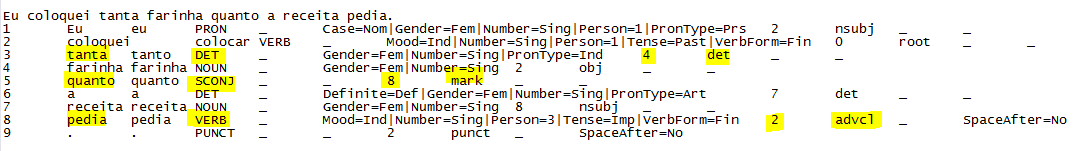
\includegraphics[width=\textwidth,height=\textheight,keepaspectratio]{imagesDrive/image20.png}
    \caption{Eu coloquei \emph{tanta farinha quanto} a receita pedia.}
    \label{fig:comparative1}
    \end{figure}{}

\begin{figure}
    \centering
    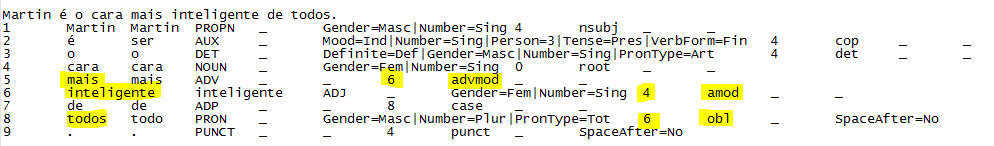
\includegraphics[width=\textwidth,height=\textheight,keepaspectratio]{imagesDrive/image27.png}
    \caption{Martin é o cara \emph{mais inteligente de todos}.}
    \label{fig:comparative2}
\end{figure}{}

\subsection{Frases do Bosque-UD}



\chapter*{Abreviações}

\hyperlink{toc}{Ir para tabela de conteúdos\\}



\chapter*{Agradecimentos}

\hyperlink{toc}{Ir para tabela de conteúdos\\}



\printbibliography[heading=subbibliography,notkeyword=this]

\end{document}
